\chapter{Machine learning foundations}

In this chapter, we aim to introduce methods of machine learning, which
are subsequently used for the purposes of predictive modelling of selected
set of stocks from the US stock market – particularly \textit{Information technology} segment.

\section{Machine learning as a method}

\section{Linear regression}

\section{Regularized variants of linear regression}

\section{k-Nearest neighbour algorithm}

\section{Random forest Algorithm}

\section{Time-series neural network (LSTM)}


\chapter{Stock market data}

The aim of this chapter is introduce set of related variables to the financial market,
their possible importance in terms of predictive modelling and lastly their subsequential
processing into specific forms, which were used through all the related analyses
in this thesis.
\par
Market itself and particularly price movement of financial instruments is a complex
and unsurprisingly counterintuitive process with a large number of more or less
related variables, which contribute to the price movement. In terms of using such data, as 
an auxiliary source, for decision making in investment strategy creation, there is a rich universe
of sources dealing with the issue \cite{clanok1}, \cite{clanok2}.
\par
%
In the thesis, we aim mainly to research predictive power of various more or less sophisticated
methods of machine learning on the particular market segment. Many papers tend to shift focus on 
single stocks or very limited set of a few stocks \cite{clanok5}, \cite{konferencia1}. Other tend to apply predicting modelling methods
on stock funds \textit{(e.g. US S}\&\textit{P 500 and NASDAQ or German DAX)} \cite{clanok4} however, there is 
a little number of sources dealing with a market segment as a whole and focus on single stocks included in it.
\par
Our main focus is on the index fund S\&P 500 – US stock index accumulating 500 biggest publicly traded companies
in terms of market capitalization. The fund itself is considered to be the most trustworthy general indicator of the overall
US and world's stock economy state \cite{snp500}. The fund itself is divided into several general market segments to which stocks belong. In this
thesis we focused on segment \textbf{Information technology} however, approach used in our analyses is adaptable to any subset of stocks –
the only determining constraint is the respective database of stocks.
\par
Information technology segment consists of $68$ US-traded stocks. As of late 2025, in terms of total capitalization, this group makes total of
nearly 30 \% of the fund, which makes it the most weighted sector, despite making only 13.6 \% of all included stocks \cite{cnbc}. This recent growth of its weight 
could be explained by a lots of factors steering the market nowadays, but the general view on the topic suggests, that recent boom of artificial 
intelligence could be the most dominant engine of growth. This suggests that focusing on this segment is wise as it could be considered the most important one nowadays.

\section{Variables in financial data}
At first, we introduce specific attributes which define value movement of all financial and economical instruments used throughout the thesis 
as feature and target variables. These attributes could be further generalised onto any financial instrument attribute's movement, not only on price 
itself – as it will be applied on non-stock data as well.
\par
For the purposes of defining desired terminology, let's define time interval on which we analyse instrument's attribute movement as $t_1$ till $t_2$, where
naturally $t_1 < t_2$. Defined atttributes, which are attached to single time breakpoints, could be universally defined for any time interval with various frequency.
\par
At the breakpoint $t_1$ we define \textbf{opening value}, which denotes value of the attribute at the very beginning of the interval. For the purposes of this thesis,
where we aim to use daily frequency of data, this value denotes value of attribute at the very start of the trading day. In the opposite manner, at the breakpoint $t_2$ we define 
\textbf{closing price}, denoting the final value of the attribute at the end of the observed interval – in our case at the end of the trading day.
\par
During the process of value evolving throughout the interval we observe global minimum and maximum of the attribute's value, which we denote \textbf{low value} and \textbf{high value} respectively.
Such data give us scent of volatility during the interval and subsequently sentiment of the market regarding the attribute.
\par
Last but not least we accumulate data regarding number of nominal instrument's stocks traded \textit{(either sold or bought)} during the time interval. This is denoted as \textbf{volume} and in terms of
the thesis this data is $> 0$ only for the stocks' data, as for some other instruments this data is irrelevant and not tracked anyhow.
\par
Last data attribute, applied only on stocks' data as well, which is strongly dependent on single stocks is volume of \textbf{dividends} paid off. Some companies oblige themselves
to pay off parts of their profit to their investors on regular basis \textit{(e.g. Apple, Microsoft or Oracle)} \cite{dividendy}. With respect to the completness of data fetched we included this data
in out potential features database.
\par
Visualisation of the terms defined on sample interval of Microsoft stock between the beginning of June 2025 and beginning of September 2025 is pictured on Figure \ref{fig:2.1}.

\begin{figure}
    \centering
    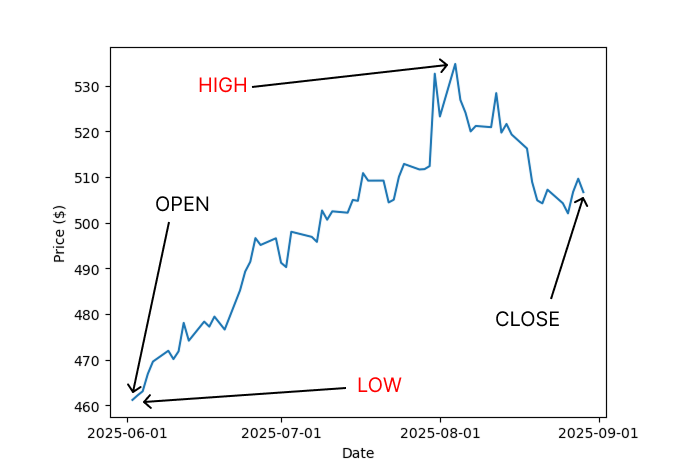
\includegraphics[width=0.9\linewidth]{images/TermsVisual.png}
    \caption{\centering \textit{Visualisation of the defined attribute's movement terms on Microsoft stock price.}}
    \label{fig:2.1}
\end{figure}

\section{Rolling window methodology}

There are quite a few approaches on how to properly process time-series data into respective training, validation and test sets. In order to ensure
intraday prediction, which means that using trading days $t-p$, $t-(p-1)$, ..., $t-1$ we predict the price value of financial instrument on the $t$ day,
we can use the methodology of \textbf{rolling window} or commonly named as \textbf{sliding window}.
\par
In this approach we define static time-series interval, which will serve as a hybrid train-validation time interval. Let's define the overall data interval being between
$T_1$ and $T_1+M$ breakpoints, meaning the overall length of the interval is $M$ \textit{(global interval)}. On this interval reside two frames of variables – possibly multivariate $Feature$ which serves 
as a input variable and univariate $Target$, which accumulates values of the predicting variable. Further, we define parameters $p<M$, which is the length of training subwindow \textit{(look-back parameter)}
and $w$, which denotes time units beyond which we aim to determine predictions. For the purposes of this thesis and its intraday prediction methodology we define $w=1$, but in general auto-regressive
case $w\geq1$ is acceptable. 
\par
For the purposes of machine learning context of feature and target variables, we denote single pieces of input and output variables as $\mathbf{X}_i$ and $Y_i$ respectively.
Using the defined parameters, division of the global interval is performed as: 

\begin{center}
\begin{minipage}{0.5\textwidth}  % Control width for centering
\begin{algorithmic}[H]  % [1] adds line numbers

\For{$i = T_1$  to $T_1+M-(p+w)$}  % Example for loop
    
$X_i \gets Feature[i, i+p]$

$Y_i \gets Target[i+p+1, i+p+w]$

\EndFor
\end{algorithmic}
\end{minipage}
\end{center}

From the rolling window algorithm pseudocode above a few imporant properties of this method could be derived.
Firstly, respective intervals are overlapping and the shift between respective $\mathbf{X_i}$, $\mathbf{X_{i+1}}$ 
and its $Y_i$, $Y_{i+1}$ is $w$, in our particular case the single time unit. Secondly, by ensuring overlapping, we maxime
number of possible training, thus validation, data points making the training-validation process possibly more robust and general.
\par
This methodology could be straightforwardly implemented to the stated problem. Further, it is sufficient to define process of
maintaining chronology in the data.

\section{Data chronology and prediction methodology}

Approach, implemented in the thesis, uses prediction based on historical developments of selected feature variables
from financial and macroeconomical markets. In order to implicitly simulate flow of time in timeseries we introduce particular 
backward shifts, using which we create setup of the modelling according to above defined constraints.
\par
Rigorously speaking, assume that method capable of predicting closing price in the day $t$ is a function, where input is movements 
of selected features in days $t-1$, $t-2$, ..., $t-p$. Let's denote the function $f$. Straightforwardly, the overall setup in general, but
the most importantly in the thesis, could be defined as:

\begin{equation}
    \label{equation:2.1}
    f(\mathbf{X}_{[t-p, t-1]}) = \hat{Y_{t}},
\end{equation}

where $\mathbf{X}_{[t-p, t-1]} \in \mathbb{R}^{p \times t}$, $p>1$ is the look-back parameter and $t\geq1$, number of feature variables used, denotes  historical developments
of selected features in the interval $t-p$ till $t-1$ and $\hat{Y_{t}}$ denotes the targeting price prediction of the instrument in time $t$.  
\par
% Tu som skončil
In accordance with the algorithm adapted for the rolling window data derivation, it is wise to implement data preparation in accordance with it. Aligned with the (\ref{equation:2.1}),
when predicting particular instrument's price in time $t$, we require having features' developments through interval of $t-p$ till $t-1$. Maintaining this, in terms of implementation, for every single
unit of time in given global interval and for every single feature, we attach its historical development up to the look-back parameter $p$. In terms of algorithm:

\begin{center}
\begin{minipage}{0.5\textwidth}  % Control width for centering
\begin{algorithmic}[H]  % [1] adds line numbers

\State $FEATURES \gets [F_1, F_2, ..., F_t]$

\For{$i = 1$  to $t$}  % Example for loop
    \For{$q = 1$ to $p$}

        $F_{i,q} \gets F_{i}$ shifted by $q$
        \EndFor
\EndFor
\end{algorithmic}
\end{minipage}
\end{center}

where $F_i, \> i \in \{1, 2, ..., t\}$ denotes single features selected for the model and $F_{i,q}$ denotes shift of the $i$-th parameter backwards
by $q$ units. With such shifted data series for every single feature, we build data points available in single days of the global interval. In rigorous manner, every single trading day $t$
has attached processed features respective to it as:
\begin{equation*}
    \forall i \in \{1, 2, ..., t\} \>  \forall q \in \{1, 2, ..., p\}: \mathcal{T}_t\gets F_{i, t-q},
\end{equation*}

where $\mathcal{T}_t$ denotes universe of model input data available at day $t$. By combining this algorithm and preparation of rolling window samples we obtain datasets in accordance with safe work with time series,
in terms of chronological sequencing, and suitable for applying predictions based on (\ref{equation:2.1}).

\section{Suitable features in modeling}

The amount of variables, which are directly or indirectly being generated together with 
day-to-day market running, is quite enormous and one should consider subsetting them 
for the machine learning purposes wisely. In this subchapter we aim to show and justify 
process of our general feature selection, mostly based on apriori knowledge of processes within
financial markets and variables' most likely effect on stock markets.
\par
For the sake of completness, data were obtained from the API directly fetching data
available on Yahoo Finance – available through Python library abstraction as \texttt{yfinance} library \cite{yfinance}, \cite{yahoo}.

\subsection{Stock indices}

In order to process current general state of the stock exchange we researched possibilities of
implementing data regarding price development of certain index funds. \textbf{Index fund} is a abstract 
concept of accumulating information regarding single stock assets into one unified asset, mostly using predefined
weighted average of prices of stocks included.
\par
Fund is specifically designed to follow and replicate performance of given subset of stocks. Taking this into account,
by including such well chosen funds, which copy broader and various scope of stocks on given market, we may obtain valuable
information regarding current state of the US market.
\par
For these purposes we decided to include into our database two major stock indices. General index \textbf{Standard's and Poor 500}, commonly
known as S\&P 500, is an index including 500 biggest US-traded stocks based on total market capitalization. Index consists of wide scope of various
segments making it robust and universal in terms of mirroring overall US market state.
\par
Taking into account the scope of this thesis – Information technology segment, we decided to include index \textbf{NASDAQ Composite}, better known as NASDAQ. The main
difference to S\&P 500 is its segment focus. NASDAQ focuses mainly on tech and IT companies, making it possibly a valuable piece of data to our
database of feature data.  

\subsection{Commodities}

Commodities denote mainly raw resources and materials, which are traded mainly in uniform quality and large quantities. Its fundamental role in the market
comes from the fact, that most of these assets play essential part in further processings, consumption and industry. Matsumoto et al. suggest, that commodity
market plays a vital part in whole financial segment, which suggests, that including such assets in database might be sufficient \cite{clanok3}.
\par
For the purposes of this thesis we included data regarding two major commodities – \textbf{crude oil} and \textbf{gold}. Even though, there might not be a clear
connection to the IT sector, we believe that such data would bring valuable information about the general state 
in the whole global economy.
\par
Oil plays a vital role in \textit{keeping the world in motion} and a solid majority of world's activities depend on its presence and availability.
This might imply, that these dependecies on the global market would be projected into price movement of the commodity.
\par
Last but not least, we introduce gold price movements into the database. With the wide range of reasons, gold still remains as one of the most
prominent securities. Most modern currencies are dependent on system, where gold acts as a security stabilizing currency movements and limiting
governments issuing money. On top of that, governments rely on physical gold as a reserve in times of crises \cite{gold}. Taking these reasons into account, 
by including gold in the database of features, we assume obtaining valuable information regarding world's economy state, crisis potential or investors' sentiment etc.

\subsection{Currency pairs - FOREX}

Currency pairs and subsequently \textbf{Foreign Exchange Market} (FOREX) denote specific market, where the main traded goods are currencies. Traders involved in the market speculate 
on certain exchange pairs volatility and bet on them in order to make profit. Market itself determines
price of every possible currency pair, thus making acquisition of certain amount of currency possible through various ways – currency $X$ could be
traded through currencies $Y$, $Z$, etc., making the market far more speculative than others. By the volume of instruments traded, this decentralized 
market is by far the largest market in the world \cite{forex1}.
\par
Being fully decentralized, meaning prices being determined on this market are accepted worldwide, these data could be considered as a sufficient
indicator of currency relative strength and by that indicator of particular government's and economical competitivness of certain country. Taking this into account,
we assume, that including such data inside our database would bring valuable information about international competitivness of US economy towards other major economies 
and quantitative information about relations among major economies, which is most likely important predictor for stock prices' movements.
\par
By our focus on US market, we chose including currency pairs with American dollar (\textbf{USD}) in all pairs. We chose to include so called \textbf{major currency pairs},
with respect to their overall traded volume on daily basis, according to reports published by \textbf{Bank for International Settlements} and to market's conventions \cite{bis_report}, \cite{forex1}.
\par
In particular, included pairs, together with USD, are Euro \textbf{(EUR/USD)}, Japanese yen \textbf{(JPY/USD)}, British pound sterling \textbf{(GBP/USD)}, Swiss frank \textbf{(USD/CHF)}, Australian dollar \textbf{(AUD/USD)}, Canadian dollar \textbf{(USD/CAD)} and New Zealand dollar \textbf{(NZD/USD)}.

\subsection{Other market indicators}
Apart from the introduced indicators and general assets price movement data above, there is still a vast group of
possibly valuable features, which do not fit into above defined features' groups. 
\par 
In order to track performance of US economy more precise, it is wise to include information regarding national debt to possible features. 
For this purpose we included data about \textbf{US treasury bonds}. Bonds denote financial instrument mostly long-term low-risk securities
issued by the government of the USA, where investor, in basic terms, lends money to the government in exchange for periodic fixed payments.
These bonds are futher divided based on its maturity – time within issuer obliges itself to fully repay issued money.
\par
Price movements of bonds with various maturity are considered to be a good indicator of US economy, thus stock market state \cite{clanok6}. In our database
of possible features we included bonds with maturity of 13 weeks, which belong to group of short terms bonds, and with 5 year long maturity. This kind of maturity
is on the edge between long-term and medium-term. The choice reflects needs of tracking data regarding relatively very short horizon and long one.
\par
Apart from the bond related data we considered obtaining data which are not directly financial – they are not some type of asset. We researched possibilities of
tracking sentiment of investors and market itself. We chose to include data of \textbf{Volatility Index} \textit{(VIX)}, which is a specific gauge tracking state
of US stock market it terms of volatility and sentiment of investors. 
\par
It presumably brings valuable information, which might not be included in all of the metrics described, regarding the apriori mood of the market 
and its assets risk. Its value ranges mostly up to $80$, which were considered as crisis values in years $2020$ and $2008$ and above approximately $10$, which
is considered to be relatively stable market state. Value development between the January till September of 2025 is given on Figure \ref{fig:2.2}.

\begin{figure}[H]
    \centering
    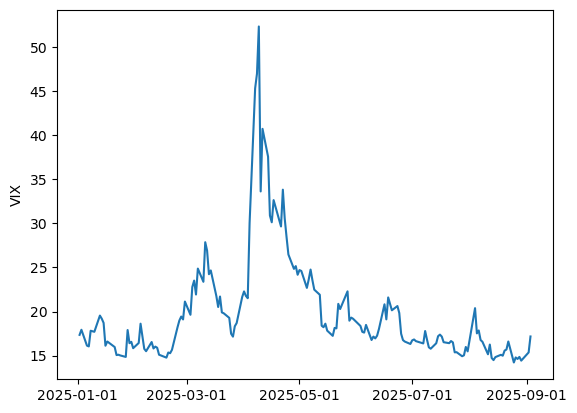
\includegraphics[width=0.9\linewidth]{images/VIX_example.png}
    \caption{\centering \textit{VIX value movement through the 2025.}}
    \label{fig:2.2}
\end{figure}

It is surely interesting to address the sudden VIX surge during the April 2025. This sudden increase was basically day-to-day and denotes 
phase of repeated issuing and cancelling of international tarrifs. As we can see, this political move damaged investors' exposure to the US market then.

\chapter{Predictive analyses on IT segment}

This chapter will be dedicated to certain results obtained during training and validation of several algorithms and approaches on the data.
We plan to analyze results brought by included algorithms in first chapter in detailed manner.

\chapter{Intraday optimization of portfolio based on model's prediction}

This chapter will deal with the topic of using the obtained data predictions \textit{(preferably from the most precise model)} to optimize weights
of single stock assets in hypothetical investment portfolio. For these purposes, we introduce Markowitz portfolio theory and the optimization 
problem coming out of it. With such foundations we analyze results in terms of profit and risk by our models.
